\subsection{Gesture Recognition}
The concept is focused on using the user as the controller and letting the movements of the user dictate how the computer should react. In order to accomplish this, knowledge of know how to make the computer understand the user’ intended action is needed. Since the concept will be camera based, then the tool for reading a user is gesture recognition.
\bigskip

\begin{figure}[h] 
\centering
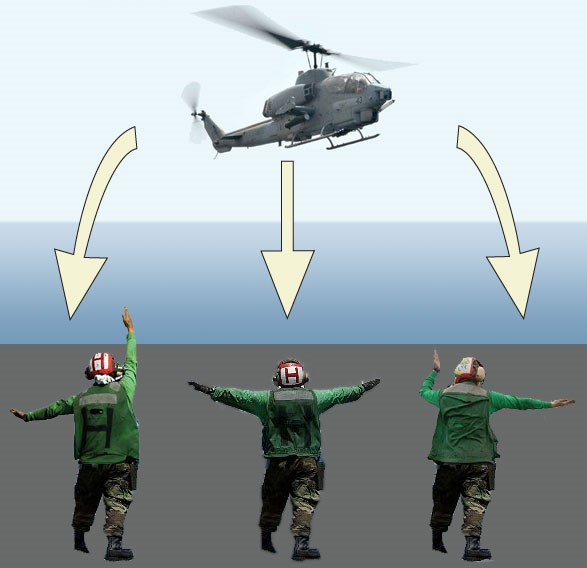
\includegraphics[scale=.33]{Gesture1} 
\caption{Gestures used to communicate instructions to a helicopter.}
\label{fig:Gesture1}
\end{figure}

\subsubsection*{What a gesture is and what they mean in relation to the concept.}
The common dictionary defines a gesture: \textit{“a movement that communicates a feeling or instruction […]”} and \textit{“to make a movement with your hands or head in order to show or tell someone something […]”}. \parencite{Macmillan2005}
This means that a general gesture is used as a form of speechless communication between two parties used to relay a message or an intent, as seen in Figure \ref{fig:Gesture1} where a movement command is being relayed to a helicopter. Gestures are often used when speech is difficult or impossible.

Because the solution will be based on a camera, then gestures will be the only viable way to communicate an intended action to the computer. Within the scope of the concept, this means that a gesture is a movement, primarily using arms or torso, which communicates an instruction to a computer to be used in an application.
\bigskip

Secondly it is necessary to know how to make a computer understand gestures given to it. For this, Image processing is needed.

The first thing that needs to be done to an image of a gesture is to isolate the gesture from the rest of the image. Some methods of doing this includes background subtraction and hue based extraction based on the hue of human skin \parencite{Busaryev}.
\bigskip

Background subtraction (section: \ref{sec:BGSub}) uses the mean values of a series of images of the same background as a basis for subtracting objects from new images. If a pixel in a new image is different enough from the mean value of the series, then the pixel can be used in a binary image of the objects. The problem with this approach is that variable conditions like lighting and noise can corrupt the results by creating false positives or objects with wrong properties. \parencite{Busaryev}
\bigskip

Another approach is hue based extraction, which converts the image to the HSV color space and then uses thresholding to detect human skin in the image. Caucasian skin has very distinguishable hue values which make it easier to detect through hue rather than regular RGB. \parencite{Busaryev}
\bigskip

A method of recognizing the gesture is the Local Feature Classifier method \parencite{Busaryev} which uses the contours of a hand and points along the contour to distinguish for example one shown finger from two and other gestures. With adjustments, this method can be used on bodies and other features.

\subsubsection*{Summary}
In summary a gesture is a movement used to communicate an instruction to a computer to be used in an application. Background subtraction or hue based subtraction, based on the hue of the skin of the user, can be used to extract a gesture from an image. The Local Feature Classifier method can be used to translate the gesture to an application command.